\documentclass[10pt]{article}
\usepackage[letterpaper,landscape,margin=0.65in]{geometry}
\usepackage{graphicx}
\usepackage[T1]{fontenc}
\usepackage{hyperref}
\hypersetup{pdftitle={Lean check of the BINSTD n=17 factor product}}
\setlength{\parindent}{0pt}
\setlength{\parskip}{0.5em}
\title{Lean check of the BINSTD n=17 factor product}
\author{Validation audit, 22 October 2026}
\date{}
\begin{document}
\maketitle
\vspace{-2em}

\textbf{Frozen source.} The BINSTD Stage-1 admissible-dimension
files agree byte for byte and list bitmask polynomials 3, 313 and 471.
The source-binding checker converts the Lean definitions back to
these exact bitmasks; the frozen file SHA-256 begins
\texttt{6f09e6c620fc}.

\textbf{Lean theorem.} In $(\mathbf Z/2\mathbf Z)[X]$,
\[
(X+1)(X^8+X^5+X^4+X^3+1)
(X^8+X^7+X^6+X^4+X^2+X+1)=X^{17}+1.
\]
The proof expands the product and reduces all even coefficients
using characteristic two. The formal task names the exact theorem;
Lean 4.35.0-rc1 reports \texttt{machine\_verified}, a passing full
build, 617 theorem declarations using only standard axioms and a
passing target audit. Independent semantic review remains pending.

\textbf{Boundary.} This checks a polynomial product. It does not prove
the degree-eight factors irreducible, identify field Frobenius with
the normal-basis polynomial module, classify every invariant
subspace or establish any empirical relation-yield ratio. The
archived toy replay is separate evidence. No performance dashboard
value or security claim changes.

\newpage
\begin{center}
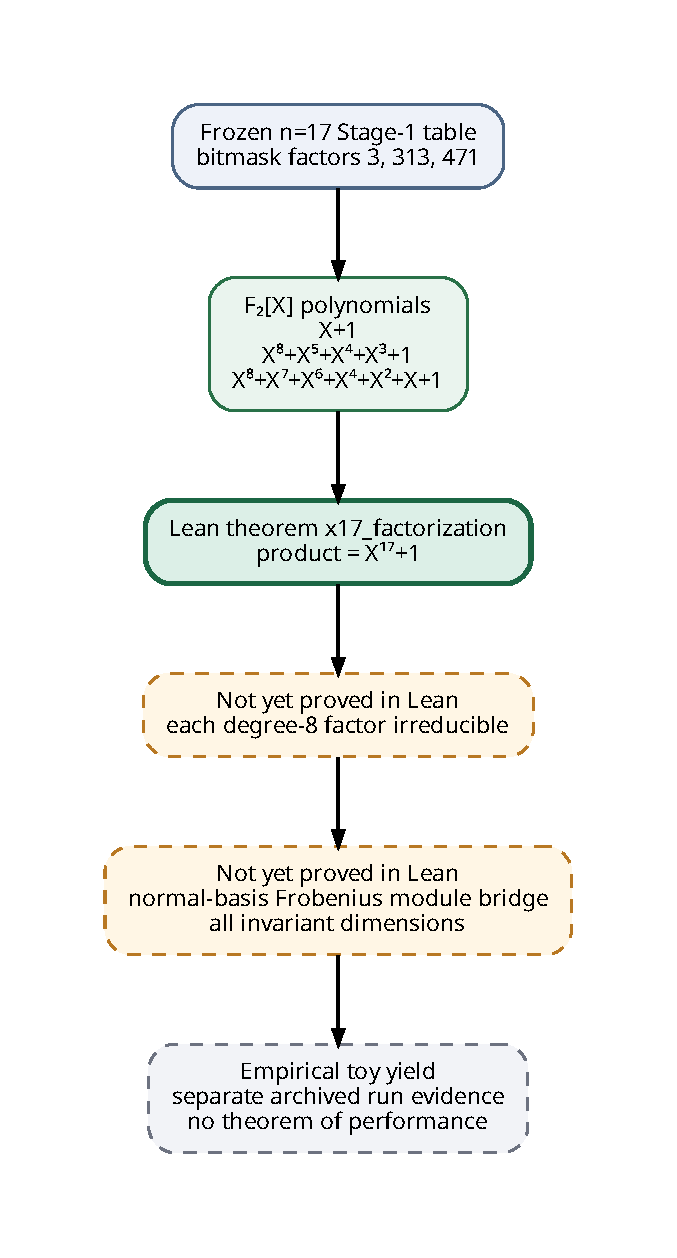
\includegraphics[width=\textwidth,height=0.82\textheight,keepaspectratio]{factorization-figure.pdf}
\end{center}
\end{document}
